\chapter{Evaluation}\label{C:evaluation}
Due to the variable nature of statistical estimation, there are several different perspectives that will be explored. Primarily, the Bayesian technique will be compared and benchmarked with the literature's competing methods. This will be analysed in terms of error between the technique's estimate BFF and the true BFF of the sample.

We evaluate the estimators via different perspectives of usability, such as : 
\begin{itemize}
    \item accuracy at the typical $T_c$ for sandstone rock and at a typical expected SNR environment given by \cite{GruberT2Estimation2013}, the target operating point of the estimator, 
    \item robustness of the estimation with respect to predicting different bound fluid cut off times, 
    \item sensitivity towards different SNR environments such that we may consider application for different noise powers, 
    \item robustness of the Bayesian estimator to different sample sizes making up the prior, and
    \item computation speed to indicate potential compatibility with different platforms.
\end{itemize}

\begin{figure}[htb!]
    \centering
    \begin{subfigure}[b]{0.49\textwidth}
        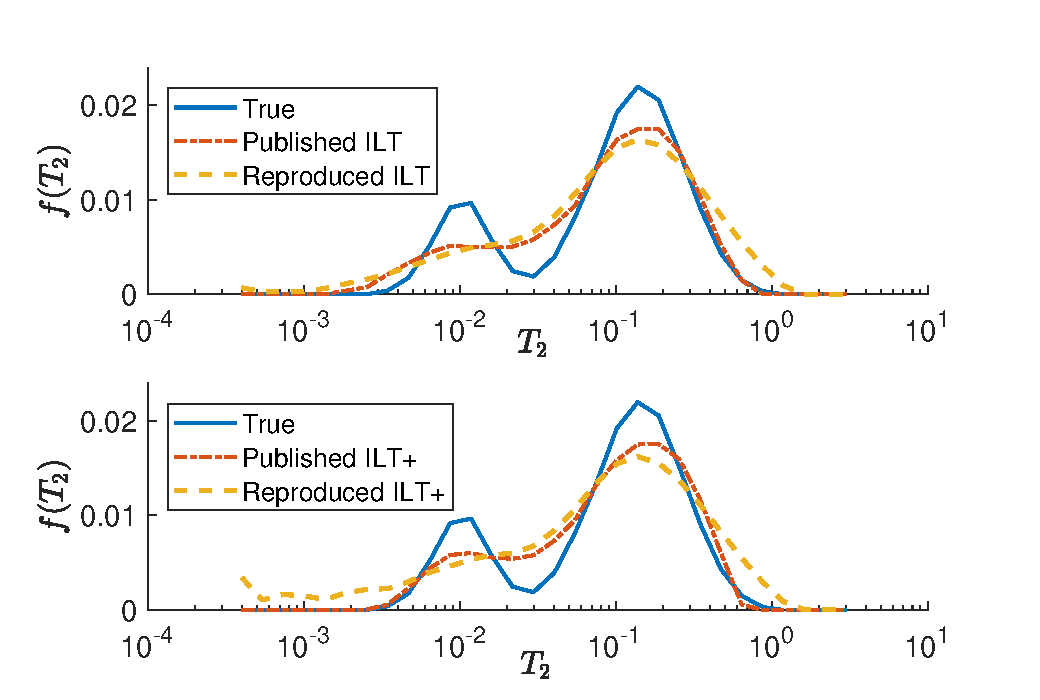
\includegraphics[width=\textwidth]{evaluation/model1_recreate.eps}
        \subcaption{Model \#1}
        \label{fig:model1Recreation}
    \end{subfigure}
    \begin{subfigure}[b]{0.49\textwidth}
        \includegraphics[width=\textwidth]{evaluation/model2_recreate.eps}
        \subcaption{Model \#2}
        \label{fig:model2Recreation}
    \end{subfigure}
    \begin{subfigure}[b]{0.49\textwidth}
        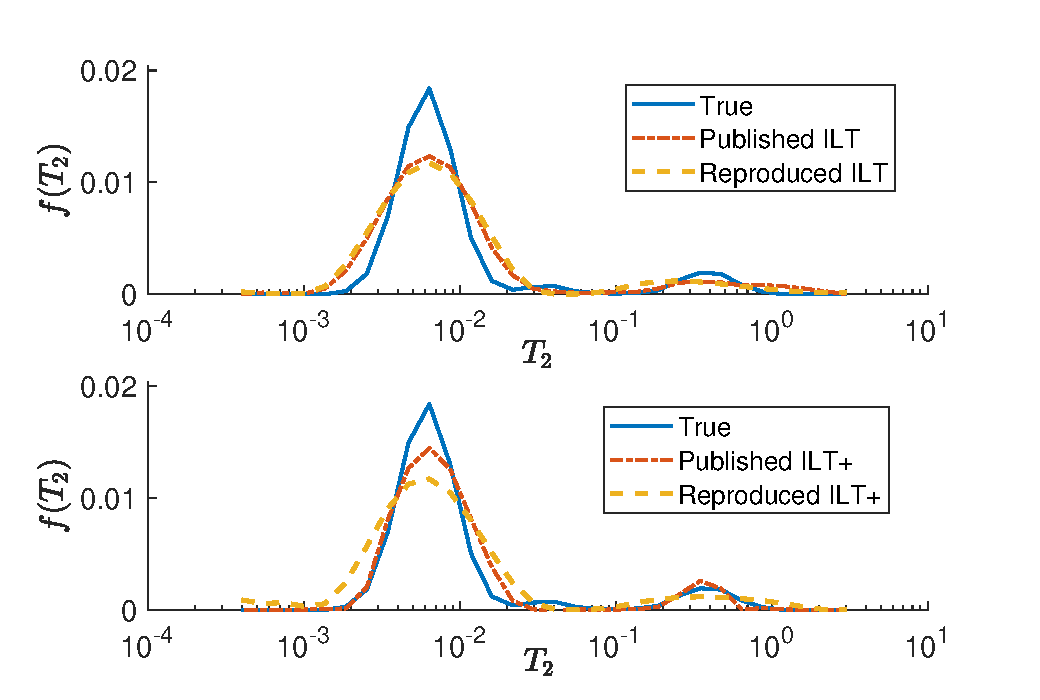
\includegraphics[width=\textwidth]{evaluation/model3_recreate.eps}
        \subcaption{Model \#3}
        \label{fig:model3Recreation}
    \end{subfigure}
    \begin{subfigure}[b]{0.49\textwidth}
        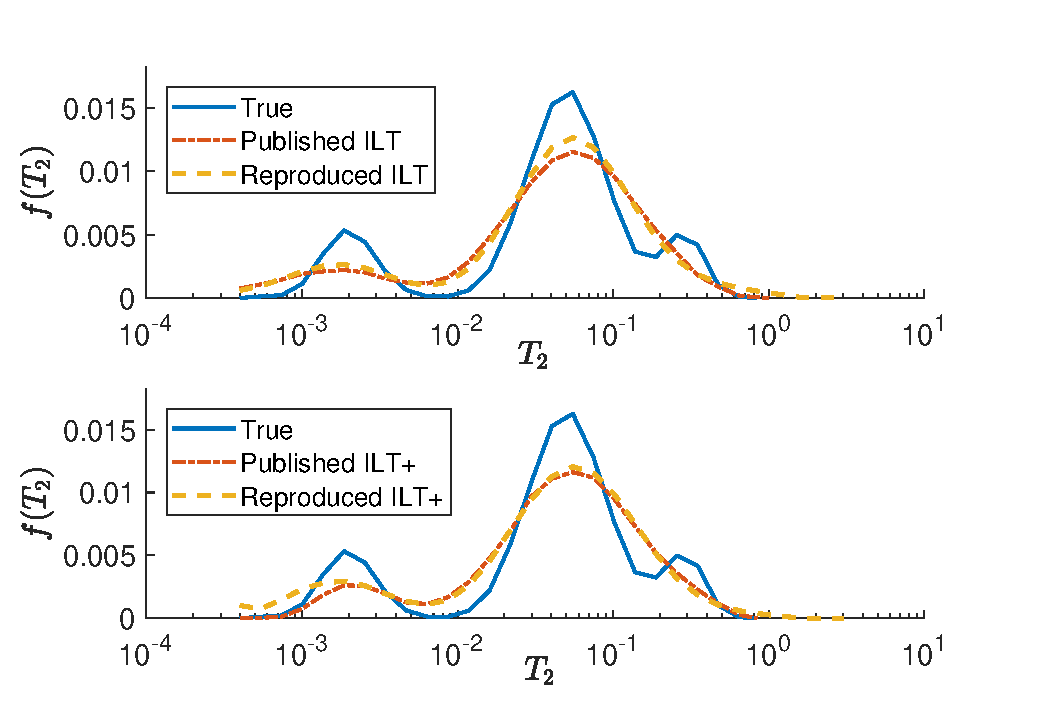
\includegraphics[width=\textwidth]{evaluation/model4_recreate.eps}
        \subcaption{Model \#4}
        \label{fig:model4Recreation}
    \end{subfigure}    
    \caption{The mean estimated $T_2$ distribution of the recreated of ILT and ILT+ methods}
    \label{fig:mean_recreated}
\end{figure}

\section{Recreated Algorithm's Closeness}
The analysis in this section utilises the same experimental conditions as detailed in \cite{GruberT2Estimation2013}. These results specifically compare algorithm recreation for an SNR of 10. The truncated singular value decomposition compression of the measurement data preserves the 10 largest singular values per \cite{GruberT2Estimation2013}.



The reproductions of the ILT and ILT+ techniques are compared with published results by Gruber et al \cite{GruberT2Estimation2013} in Figure \ref{fig:mean_recreated}. The ILT+ technique is particularly erroneous for relaxation times below 3 ms. This is likely to be an error in the implementation of the moment estimator as discussed in Section \ref{section:moment_est_implementation}. Nevertheless, the reproduced techniques, even with error in the replication of the ILT+, still provide some indication of the typical performance of these techniques.

Table \ref{tab:reproductionError} demonstrates the difference between the overall signal error in implementation and the signal power (porosity of the sample, $\phi$) of the overall estimate. We see that the error from estimation tends to be below 10\% for the typical density functions. This error does not overwhelm the estimated signal. This means that reproduced performance is indicative of the true application of the algorithm. In addition, if there is a performance gap beyond 10\% in the evaluation, it means the implementation error is unlikely to invalidate the performance comparisons made.


\begin{table}[htb!]
\centering
    \begin{tabular}{l p{1.75cm} p{1.75cm} p{1.75cm}  p{1.75cm} p{1.75cm} p{1.75cm}}
    \toprule
    	& Reprod. ILT Error $\phi_E$ & Published ILT $\phi$ & ILT Error $\frac{\phi_E}{\phi}$ & Reprod. ILT+ Error $\phi_E$ & Published ILT+ $\phi$ & ILT+ Error $\frac{\phi_E}{\phi}$  \\
    \midrule
	Model 1 & 1.13E-2 & 0.1502 & 7.52\% & 1.48E-2 & 0.1507 & 9.82\% \\ 
	Model 2 & 1.31E-2 & 0.2911 & 4.50\% & 2.3E-2 & 0.2854 & 8.06\% \\ 
	Model 3 & 9.4752E-4 & 7.3800E-2 & 1.28\% & 9.100E-3 & 6.94E-2 & 13.11\% \\
	Model 4 & 5.3E-3 & 0.1024 & 5.18\% & 7.00E-3 & 0.1013 & 6.91\% \\ 
    \bottomrule

    \end{tabular}
        \caption{Error for the mean of the reproduced ILT and ILT+ density function estimates compared to the published results' mean estimate in \cite{GruberT2Estimation2013}. The values published here are unit less in correspondence with published results.}
    \label{tab:reproductionError}
\end{table}








\section{Technique Comparison for a Chosen $T_c$} \label{section:aChosenTc_evaluation}
The analysis made here is for the typical bound fluid cutoff for sandstone: $T_c = 33$ ms \cite{UsingNMRPetrophysicalKenyon1992nuclear}. Figure \ref{fig:cdf_all_tech} illustrates an empirical cumulative distribution function (CDF) of the absolute error of the estimate bound fluid fraction. The closer the line is to the y axis, the more better it is for a given cumulative probability.

As we can see from Figure \ref{fig:cdf_all_tech}, the Bayesian estimator with the sharp BFV integral transform outperforms all of the other techniques except for at the 99\% probability point of the CDF. It has 80\% of all estimated $BFF$ below an absolute error of 0.062. Comparatively, the performance of the Bayesian estimator with the tapered BFV integral transform is close to that of the ILT method. 80\% of both the Bayesian tapered and ILT techniques have an absolute estimation error of up to 0.1200. This 50\% reduction of error at this cumulative probability indicates a strong case for the viability of the Bayesian framework.

As we move our analysis towards the 95\% probability threshold of error, the sharp BFV Bayes and ILT+ methods' performance gap becomes smaller. Specifically, the Bayes Sharp BFV has 95\% of all BFF estimations with an absolute error below 0.1295. The reproduced ILT+ in comparison has 95\% of its estimations below an absolute error of 0.1479. 

The EHT method appear to have undoubtedly the worst performance out of all of the compared techniques. This is likely due to it being the least comprehensive form of estimation. It involves only one integral transform while the other methods include optimisation or a comprehensive prior.

\begin{figure}[htb!]
    \centering
    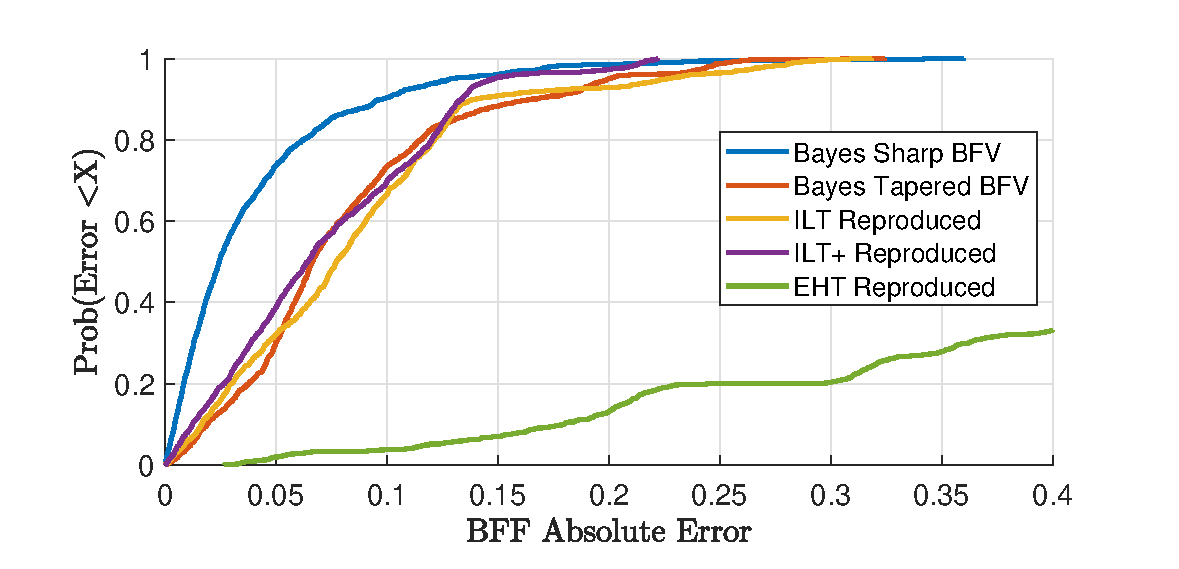
\includegraphics[width=\textwidth]{evaluation/main_analysis_plot.eps}
    \caption{Cumulative distribution function of the $BFF$ absolute error from the test architecture with respect to the experimental variables given in Table \ref{tab:test_variables}}
    \label{fig:cdf_all_tech}
\end{figure}

\section{Performance for Different $T_c$} \label{section:differentTc_evaluation}
When we expand the analysis towards a range of different cut-off times for bound fluid fraction, we notice the superior performance of the sharp BFV Bayesian estimator. Figure \ref{fig:TestDifferentTc} illustrates that the sharp BFV transform performs considerably better than the other techniques except for where $T_c$ lies between 1 ms and 6 ms. At the typical operating points of a bound fluid cut-off of 33 ms (for sandstone) and 90 ms (for carbonates) \cite{wellLoggingBook}, the sharp Bayes technique far outperforms the other techniques, by up to 0.025 in the estimation error. 

\begin{figure}[htb!]
    \centering
    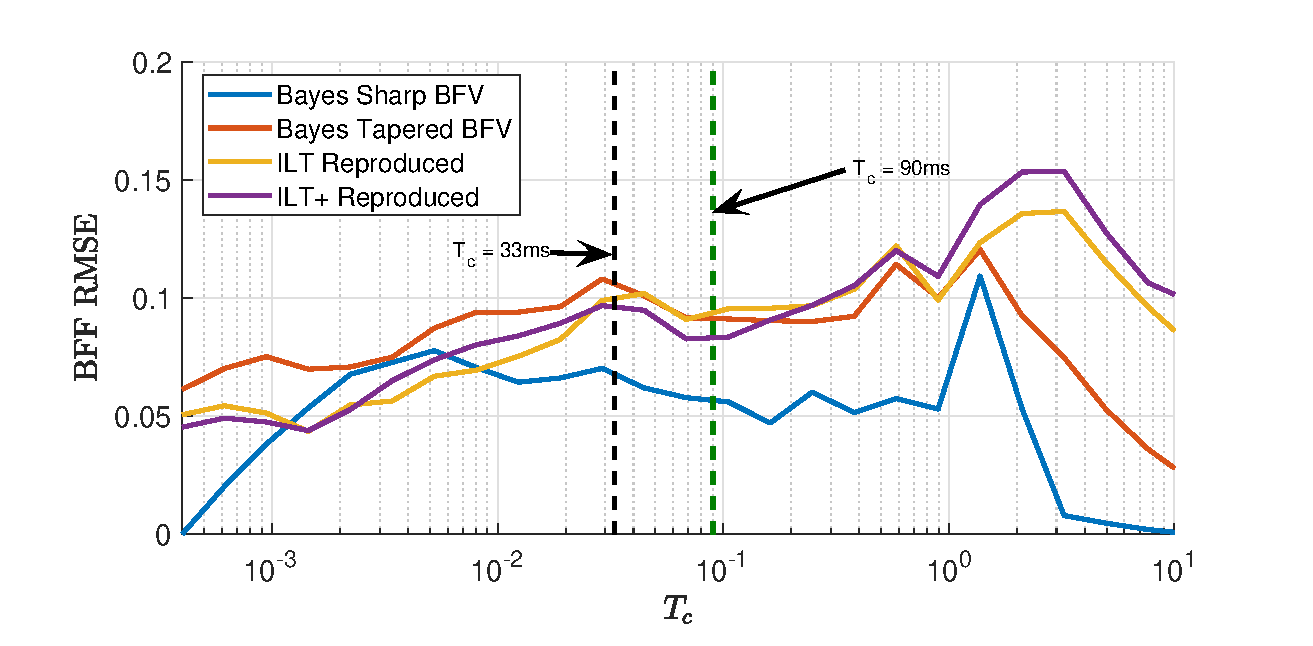
\includegraphics[width = \textwidth]{evaluation/different_Tc.eps}
    \caption{Root mean square error for different $T_c$, SNR = 10. The EHT has been omitted from this analysis to allow closer analysis of the more viable techniques}
    \label{fig:TestDifferentTc}
\end{figure}

The tapered Bayes technique in comparison performs poorly compared to the sharp Bayes technique. This implies that compensating for leaks between the T2 relaxation bins impairs performance. At no point does the tapered method outperform the sharp method. It performs closest to the sharp BFV technique in the short relaxation region of $T_c$ = 2 ms to 4 ms.

The sharp BFV Bayes estimator has an RMSE of less than 0.01 at the bounds of the T2 axis. This indicates that there is little leakage between the density function bins and hence the estimate BFF. This would be due to a near zero prior density function at these T2 relaxation times for all of the experimental density results. The other techniques have a degree of leakage between the relaxation bins that cause non-zero error in their cases. This is an operating region where the descriptive prior of the Bayesian estimator is at its most advantageous.




\section{Performance for Different $SNR$} \label{section:differentSNR_evaluation}
Estimation of the BFF will be typically done in environments with a potentially variable amount of noise power. This section of the evaluation explores how SNR affects estimation error. Figure \ref{fig:Comparative_SNR} illustrates an empirical CDF of absolute error for the techniques at different SNR values.  

We see that the sharp Bayes method  typically performs better than all of the other techniques for each of the different SNRs. For a lower SNR we observe that the sharp Bayes technique tends to perform more similarly to the ILT benchmark. The performance difference becomes more apparent at higher SNR.

As we examine the 80\% cumulative probability bound of the error, we see that that as the SNR increases, the sharp BFV Bayes estimator widens the performance gap between the competing techniques. For example, at a poor measurement SNR of 1 the error gap between the ILT and Bayes Sharp BFV is 0.0332. As the SNR increases to 100, this gap more than doubles to an error difference of 0.0766. 

We must note that as we examine performance at an increasingly high SNR, we begin to leave the scope the estimator aims to satisfy. This is because high quality experimental results are supposed to be tightly controlled and not influenced by prior information. Detailed prior information may only be suitable in noisier environments where we are unable to control much of the experiment. In those cases, we may accept the use of more detailed prior information to form an estimate. 


\begin{figure}[htb!]
    \centering
    \begin{subfigure}[b]{0.49\textwidth}
        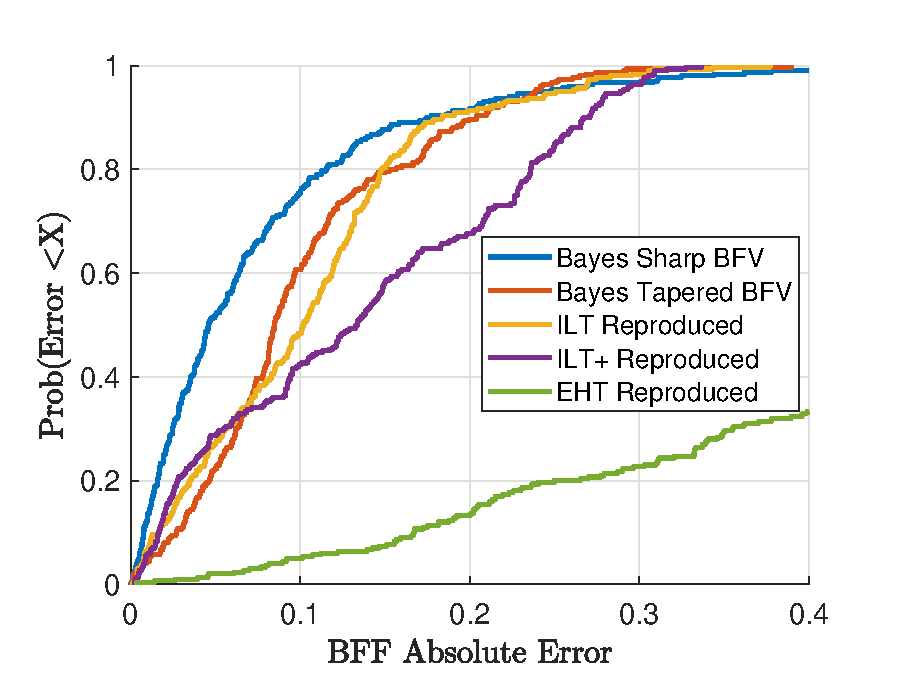
\includegraphics[width = \textwidth]{evaluation/cdf_SNR_1.eps}
        \caption{SNR = 1}
    \end{subfigure}
    \begin{subfigure}[b]{0.49\textwidth}
        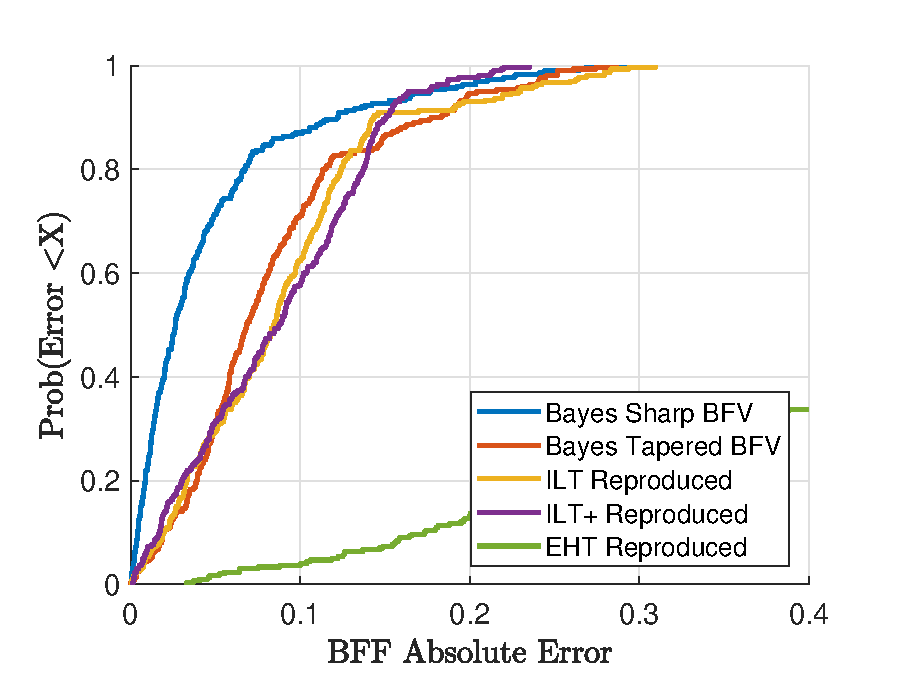
\includegraphics[width = \textwidth]{evaluation/cdf_SNR_5.eps}
        \caption{SNR = 5}
    \end{subfigure}
    \begin{subfigure}[b]{0.49\textwidth}
        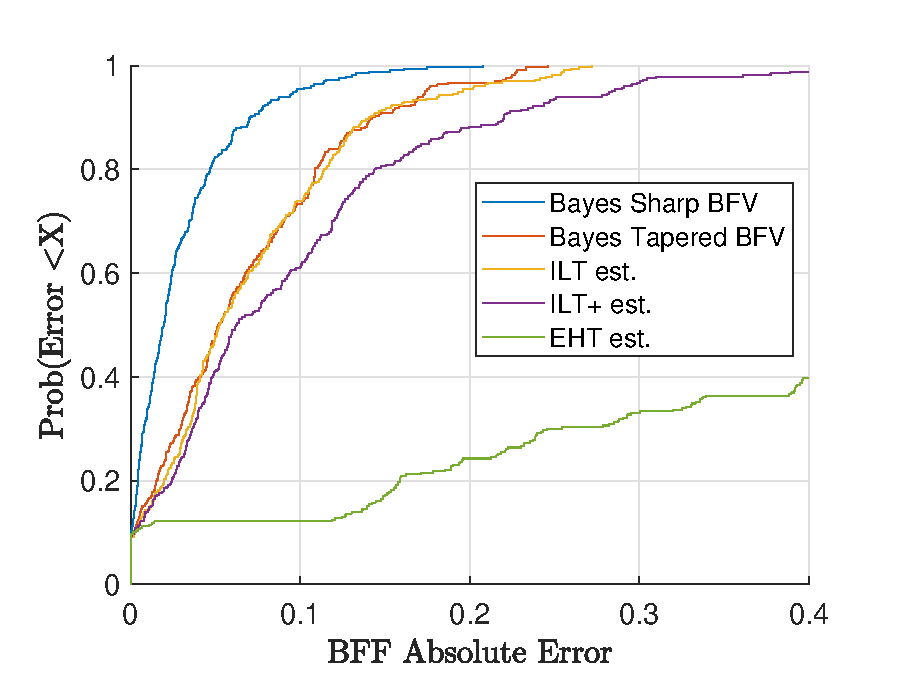
\includegraphics[width = \textwidth]{evaluation/cdf_SNR_10.eps}
        \caption{SNR = 10}
    \end{subfigure}
    \begin{subfigure}[b]{0.49\textwidth}
        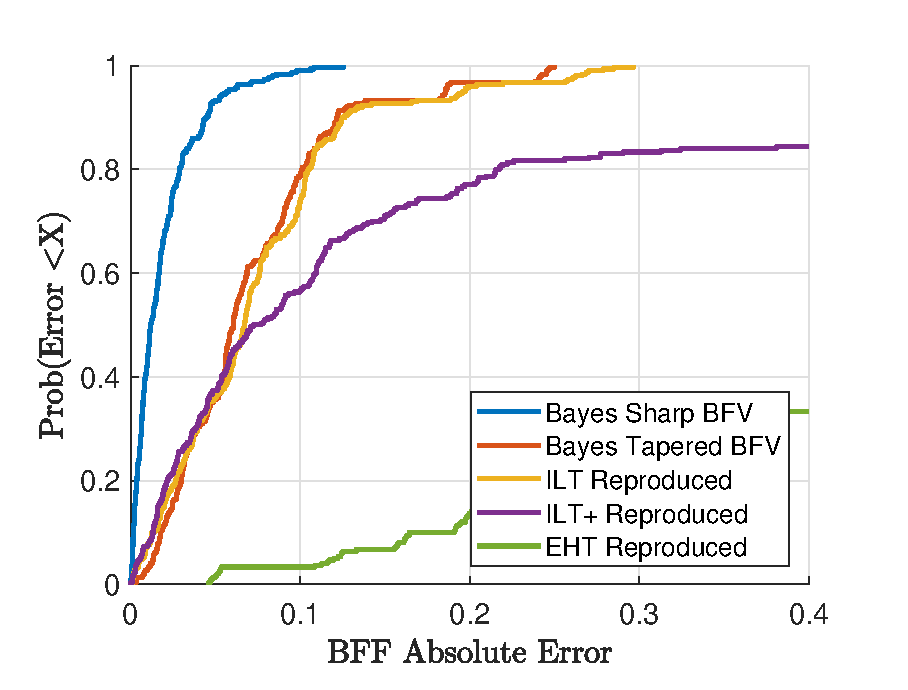
\includegraphics[width = \textwidth]{evaluation/cdf_SNR_100.eps}
        \caption{SNR = 100}
    \end{subfigure}
    \caption{Cumulative distribution functions for BFF estimation error for different SNRs}
    \label{fig:Comparative_SNR}
\end{figure}

\section{Dependence on the Prior}

A crucial element for the Bayesian estimator is its robustness to changes in the prior. Figure \ref{fig:different_prior} compares the BFF estimate absolute error for different amounts of randomly chosen density functions used to construct the prior. We explore the Bayesian estimator with a sharp BFV integral in this analysis. This was repeated via cross-validation for each of the 30 samples 50 times.

This analysis of prior generality illuminates the importance of an effective prior for the Bayesian estimator. As we increase the number of instances that make up the prior, we converge towards a performance bound with diminishing returns. The benefits of an increase to a prior's sample size is pronounced for an increase from 5 to 10 density functions. 50\% of the absolute error is below 0.070 for a prior built from 5 instances. The prior constructed with 10 experimental instances has 50\% of the absolute error below 0.029. This decrease of error by 58\% at this cumulative probability emphasises how a more detailed prior is important for the Bayesian estimator.

The reproduced ILT+, the best of the existing reproduced techniques, tends to generally outperform the Bayesian estimator for where there are 5 or less experimental density functions forming the prior. As the sample size decreases, the Bayesian technique becomes progressively worst as it loses generality. In addition, the Gaussian assumption of the prior density function is less reasonable at these small sample sizes. This exemplifies the Bayesian framework's limitations for generality for where there is little experimental data to form the prior.

\begin{figure}[htb!]
    \centering
    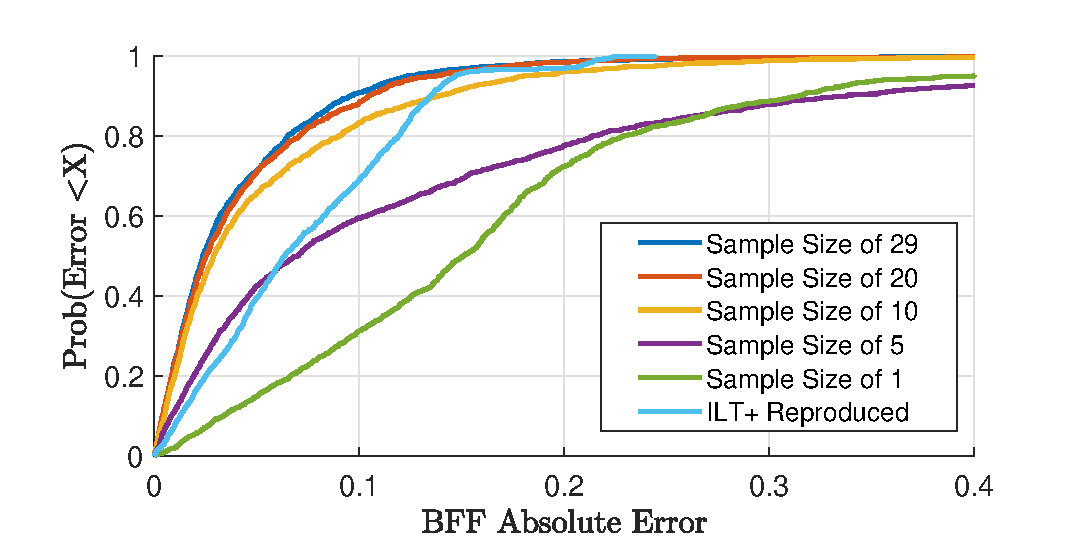
\includegraphics[width=\textwidth]{evaluation/different_priors.eps}
    \caption{CDF comparison of Bayesian estimation absolute error for different numbers of randomly chosen instances forming the prior}
    \label{fig:different_prior}
\end{figure}

\section{Computation Comparison}
Figure \ref{fig:computation_time_results} demonstrates the difference in computation time for each of the techniques. Generally, we see that the proposed Bayesian techniques takes consistently longer than all of the other techniques due to the absence of compressive preprocessing.

The EHT outperforms all of the other techniques, as it requires no matrix inversion or any iterative computation. This comes at the trade off in terms of actual accuracy as demonstrated in Sections \ref{section:aChosenTc_evaluation} - \ref{section:differentSNR_evaluation}. This means it is served best augmenting another method such as the ILT+ rather than being its own standalone estimator.

The ILT and ILT+ are comparable as they contain the intensive singular value decomposition of (\ref{eq:compressedMeasurement}) and multiple matrix inversions of the compressed matrix in (\ref{eq:optFindC}). A matrix inversion has a high computational complexity \cite{invertMatrixComputational}, so if the dimensionality is reduced significantly, performance is decisively increased.

The Bayes method is the slowest as even though there is no iterative computation, it involves the inversion of a term that contains the uncompressed kernel (\ref{eq:posteriorProbability}). This expensive computation implies that compressing the input in some way before introducing it into the framework potentially would yield a better computation speed.


\begin{figure}
    \centering
    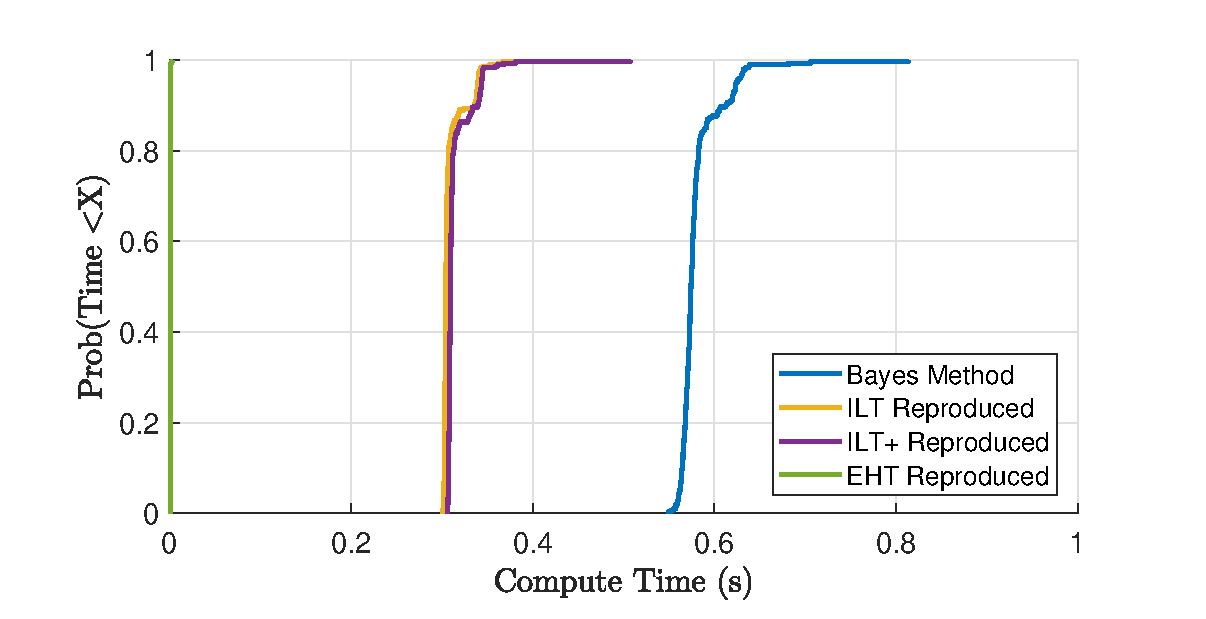
\includegraphics[width = 0.8\textwidth]{evaluation/compute_time_compare.eps}
    \caption{Cumulative distribution functions of computation times for each of the techniques}
    \label{fig:computation_time_results}
\end{figure}

\iffalse
\begin{table}[]
\centering
\begin{tabular}{l c c c c}
\toprule
                      & EHT       & ILT    & ILT+   & Bayes  \\ 
\midrule
Median Time (seconds) & 7.881E-04 & 0.3041 & 0.3093 & 0.5741 \\
\bottomrule
\end{tabular}
\caption{Computation time statistics for the different estimation techniques}
\label{tab:computationTimes}
\end{table}
\fi

\section{Evaluation Conclusions}
We have determined that given a prior that is representative of what is being estimated, we may estimate the BFF more accurately with the Bayesian estimator. This has been demonstrated for different SNR and different bound volume cut-off times ($T_c$). However, it is outperformed in terms of computation due to the lack of compression in the framework and is heavily dependent on its prior. Given that experimental data may be available for potential users of this estimator, the latter is less of a concern. The actual performance of the Bayesian technique for these different performance metrics forms a strong case for its viability and use.